\newpage
\section{Die Bewaffnung}
\subsection{G36-Visier}
Seit wir das G36 haben, haben wir auch endlich wieder vernünftige Markierungen im optischen Visier. Damit braucht ihr als Schütze auch keine Rangefinder mehr - das ist alles <<all-ink>>. Erklärung anbei. Bei uns sieht die Strichplatte etwas anders aus, die Funktionen sind die gleichen. \\
\begin{minipage}[t]{1\textwidth}
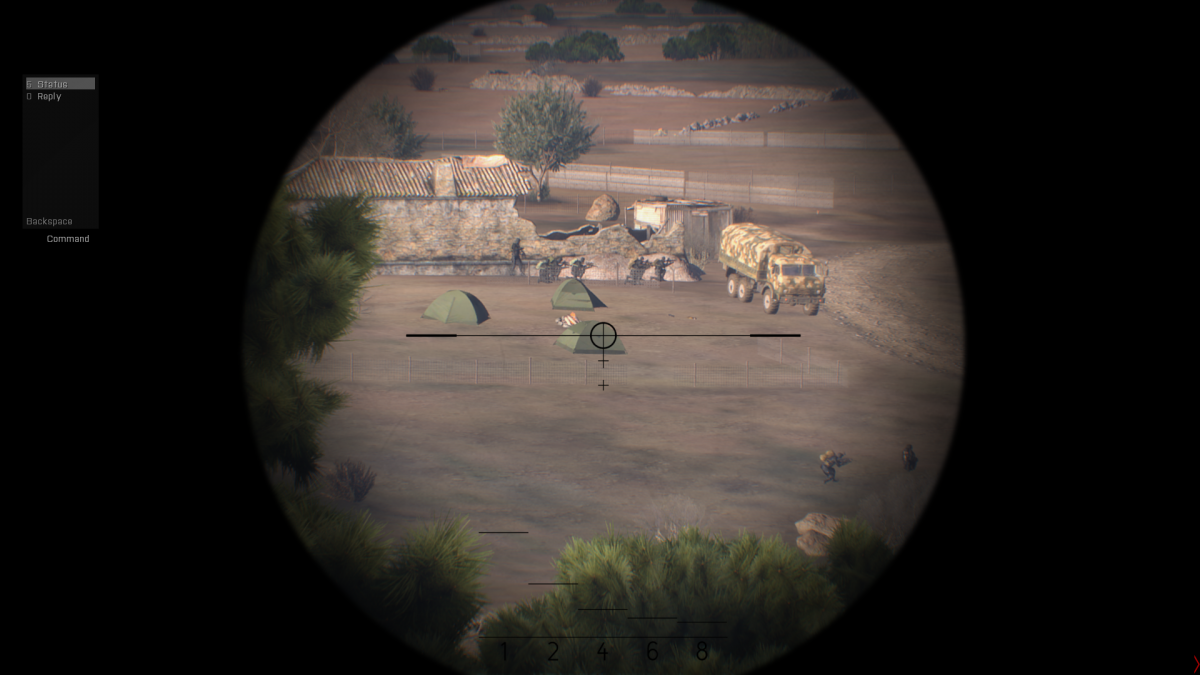
\includegraphics[width=\textwidth]{./Grafiken/Abschnitt/G36_teaser.png}
\end{minipage}
\begin{minipage}[t]{1\textwidth}
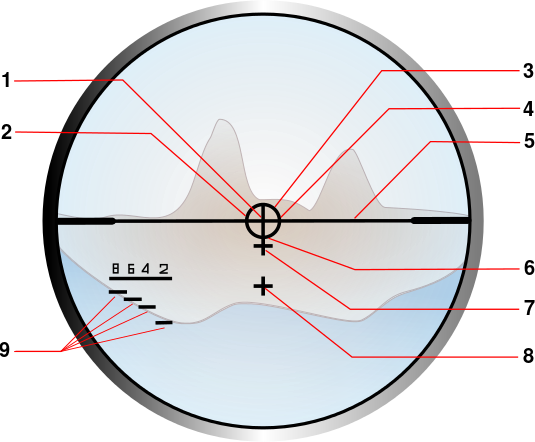
\includegraphics[width=\textwidth]{./Grafiken/Abschnitt/G36_Visier.png}
\end{minipage}
\begin{enumerate}
\item Zielmarke 200 m
\item Vorhaltemarke links bei Zielgeschwindigkeit von ca. 8 km/h bei 200 m Entfernung
\item Zielkreis (Innerer Durchmesser Schätzmarke 1,75 m Zielhöhe auf 400 m)
\item Vorhaltemarke rechts bei Zielgeschwindigkeit von ca. 8 km/h bei 200 m Entfernung
\item Horizontale Linie zur Verkantungserkennung
\item Zielmarke ca. 400 m
\item Zielmarke 600 m
\item Zielmarke 800 m
\item Entfernungsschätzmarken für Zielhöhe 1,75 m bei Entfernung X (200, 400, 600, 800m)
\end{enumerate}

\subsection{Das G36}
Das G36 ist eineStandard Infanterie Waffe. Ihre optimale Einsatzreichweite liegt bei ca. 100-400 m \\
Grenadiere, Truppführer sowie ihre Funker verfügen über ein G36 mit zusätzlichem Unterlaufgranatwerfer. Dieser wird durch umschalten mit der Feuermodi Taste (F) erreicht. Durch drücken von \glqq Bild hoch\grqq und \glqq Bild runter\grqq wird die Entfernung eingestellt (50-350 m). Der Unterlaufgranatwerfer stellt damit eine hervorragende Waffe da um Feindverbände zu unterdrücken und weiter entfernte Ziele mit Rauchgranaten zu markieren. \\

\subsection{Das MG5 (HK121)}
Das Maschinengewehr 5 wird im Verbund mit einem MG Assistenten eingesetzt. Das MG5 ist eine der effektivsten Waffen zur Infanteriebekämpfung. Das Visier entspricht dem G36. Seine schwere 7,62 mm Munition kann auch Gebäude oder leichte Deckung durchschlagen. Bevorzugt sollte das MG5 im Liegen und aufgelegt eingesetzt werden. Der MG-Assistent trägt die Munition und sichert den MG-Schützen mit ab. Das MG5 verfügt über drei Feuermodi, die unterschiedliche Feuerraten und damit unterschiedliche Präzision anbieten.  (ca. 600  / 700 / 800 Schuss /min) \\

\subsection{Das Panzerfaust 3 Visier}
Die Panzerfaust 3 ist unsere Standard AT (Anti-Tank) Waffe und wird gegen stark gepanzerte Fahrzeuge eingesetzt. Im Visier sind 5 Distanzmarken eingezeichnet. Von Unter 100 - 400 Meter. Die Panzerfaust 3 wird rein optisch gezielt, es gibt keine Zielführung oder "Lock On" wie bei manchen anderen AT Waffen. \\
 Ein statisches Ziel sollte zwischen den linken und rechten Balken möglichst eingegrenzt werden, so dass das Mittlere + etwa auf der Höhe des Turms ausgerichtet ist. Ist das Ziel im Nahbereich (< 100m), genügt es das oberste, eingekreiste Plus bzw. dessen Führungslinie zu verwenden. Bewegt sich das Fahrzeug nach Links oder Rechts weg, ist das jeweilige der Richtung entgegensetzte + zu verwenden, da das Geschoß je nach Distanz verzögert eintrifft. \\
\begin{minipage}[t]{1\textwidth}
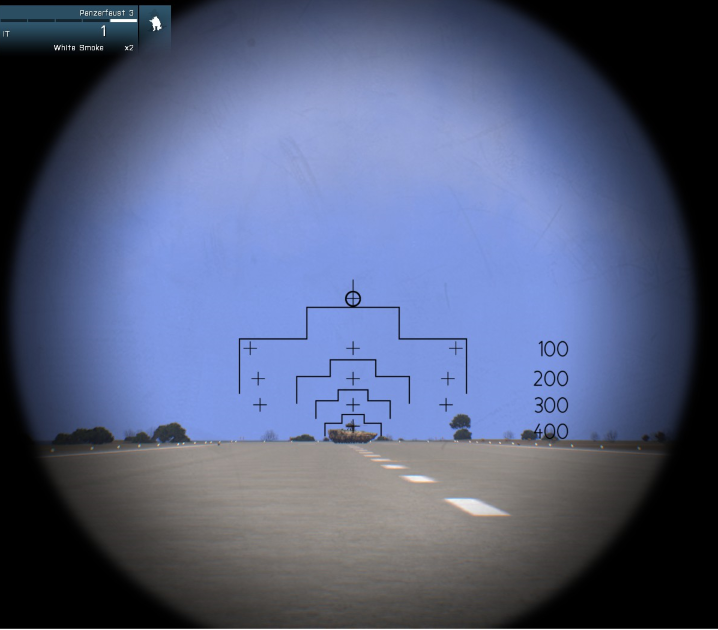
\includegraphics[width=\textwidth]{./Grafiken/Abschnitt/Panzerfaust_Visier.png}
\end{minipage}

\subsection{Die Panzerfaust 3}
Die Panzerfaust 3 ist eine Einwegwaffe. Zur Reduzierung der Sichtbarkeit kann der Gefechtskopf beim Transport entfernt werden. Beim Einsatz der Panzerfaust 3 ist zu beachten dass diese eine Rückstrahlzone hat in der befreundete Einheiten verletzt werden können. Diese Rückstrahlzone ist minimiert aber vorhanden. Um sicherzustellen das keine befreundeten Einheiten sich in dieser Rückstrahlzone befinden wird die PZF3 auf das Ziel ausgerichtet und gefragt ob die 
\glqq Rückstrahlzone frei?\grqq ~ ist. Anwesende Einheiten überprüfen dann ob diese frei ist und geben dann die Freigabe \glqq Rückstrahlzone frei!\grqq. Die Panzerfaust bleibt dabei immer auf den Feind (oder erwarteten Feind gerichtet).  Mit der Panzerfaust 3 kann fast jedes Fahrzeug mit einem Schuss zerstört werden. \\

\subsection{Das Fliegerfaust 2 Stinger Visier}
Die Fliegerfaust ist unsere Standard \acf{AA} Waffe. Sie wird vor allem gegen niedrigfliegende feindliche Hubschrauber und Drohnen eingesetzt, kann aber auch gegen Flugzeuge wirken. Ihre Maximalreichweite beträgt ca. 6km, die maximale Flughöhe des Ziels ist < 2km. \\
Die Fliegerfaust hat ein relativ simples optisches "Guckloch" Visier, welches zur optischen Zielerfassung dient, jedoch nicht unbedingt für die Zielerfassung erforderlich ist. Für die Zielerfassung wird ein "Lock-On" System verwendet, sprich man muss die Fliegerfast auf das Ziel ausrichten, danach drückt man T (Lock Target Taste) und erhält einen wiederholenden Ton, der anzeigt, das das Ziel erfasst wird. Sobald die Fliegerfaust das Ziel endgültig erfasst hat erhöht sich die Frequenz und Wiederholrate dieses Tons und man kann den Abzug betätigen. Je weiter ein Ziel entfernt ist, desto wirksamer sind die vom Ziel eventuell eingesetzten Gegenmaßnahmen, es empfiehlt sich generell immer sofort nachzuladen und einen nachfolgenden Schuss abzusetzen. \\
\begin{minipage}[t]{1\textwidth}
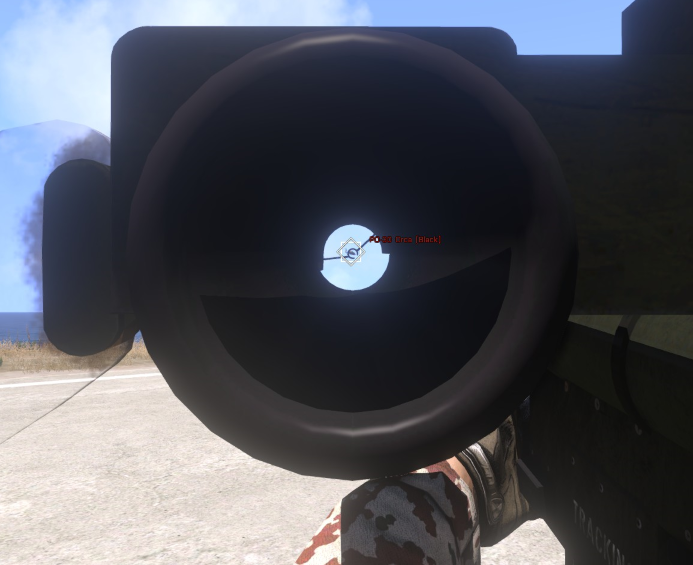
\includegraphics[width=\textwidth]{./Grafiken/Abschnitt/Fliegerfaust_Visier.png}
\end{minipage}

\subsection{Die Fliegerfaust}
Sie wird selten im \ac{TTT} eingesetzt da die meisten Terroristischen Feindverbände über keine Flugeinheiten verfügen bzw. diese durch die Flugeinheiten bekämpft werden. Es gelten die gleichen Regeln für die Rückstrahlzone wie bei der Panzerfaust 3.\\

\subsection{Granaten}
Jeder Infanterist verfügt über Spreng-, Rauch-, Blend- und \acf{IR}-Granaten. Zusätzlich (Aufgrund der Verwendung) Knicklichter. Der Einsatz von Granaten sollte sorgfältig überlegt sein. \\
Rauchgranaten sollten entsprechend ihrer Rauchfarbe eingesetzt werden. Individuell kann ein anderer (Farb-) Einsatz abgesprochen werden. Ein kleiner Hinweis das man, und auch welche, Granate man einsetzt hat sicherlich noch niemanden geschadet. Ein typisches Problem ist auch das Rauchgranaten eher zu selten als zu oft eingesetzt werden. \\
\\
\begin{tabular} {|p{0.25\linewidth}|p{0.65\linewidth}|} \hline
Roter Rauch		& Markierung von Feinden\\ \hline
Grüner Rauch	& Markierung der eigenen Stellung \\ \hline
Grauer Rauch	& Einnebeln der eigenen Stellung um unerkannt anzugreifen oder sich zurückzuziehen\\ \hline 
Violetter Rauch & Markierung von Landezonen \\ \hline
\end{tabular}\\
\\
\ac{IR}-Granaten dienen der Markierung von Gebieten (bei Nacht) um zum Beispiel \ac{CAS} einzuweisen. \ac{IR}-Granaten sind deutlich sichtbar für jedes Nachtsichtgerät! \ac{IR}-Granaten und Knicklichter können auch mittels \ac{CSE} Menü am Körper angebracht werden.

\subsection{Sonderbewaffnung}
Sonderbewaffnung sind den Spezialisten Trupps überlassen und stellen damit nicht den Teil der \ac{AGA} dar. Sonderbewaffnungen bedürfen einer Speziellen Grundausbildung (\ac{SGA}). Erwähnt seien hier die Minen und Sprengsätze von Pionieren, Drohen der \ac{UAV}-Operatoren, Scharfschützengewehre und Mörser. \\


